\documentclass[a4paper]{article}
\usepackage{hyperref}

\title{HANDBOOK V2 : \\ \textbf{Everything you need to know} \\ Master level}
\author{Florentin Julien}
\date{}



\usepackage[left=3cm,right=3cm,top=3cm,bottom=3cm]{geometry}

\usepackage[english]{babel}
\usepackage[utf8]{inputenc}
\usepackage[T1]{fontenc}
\usepackage{tikz}
\usepackage{pgfplots}
\pgfplotsset{compat=1.18}
\usepackage{xcolor}
\usepackage{ragged2e}
\usepackage{array}
\usepackage{multicol}
\usepackage{diagbox}
\usepackage{multirow}
\usepackage{cancel}
\usepackage{slashbox}
\usepackage[most]{tcolorbox}
\usetikzlibrary{calc}
\usepackage{amssymb}
\usepackage{fourier}
\usepackage{subfiles}
\usepackage{tocloft}
\usepackage{etoc}
\usepackage{draftwatermark}

\newcounter{mastersem}
\setcounter{mastersem}{0}

\newcounter{numdisplay}
\setcounter{numdisplay}{0}

\SetWatermarkText{}
\SetWatermarkScale{0.5}  % Adjust the scale as needed
\SetWatermarkColor[gray]{0.3}  % Adjust the color as needed

%%%%%%%%%%%%%%%%%%%%%%%% VALUES TO CHANGE %%%%%%%%%%%%%%%%%%%%%%%%%%%%%%%%%
\newcounter{isFree} %admin power variable
\setcounter{isFree}{1} %if isFree = 0 then add watermark and remove courses, else remove it

\newcounter{MA1}
\setcounter{MA1}{0}
\newcounter{MA2}
\setcounter{MA2}{0}
\newcounter{MA3}
\setcounter{MA3}{0}


%%%%%%%%%%%%%%%%%%%%%%%% END OF VALUES TO CHANGE %%%%%%%%%%%%%%%%%%%%%%%%%%%%%%

\newcounter{bought1}
\setcounter{bought1}{0} %if bought1 > 0, remove watermarks on ToC

\addtocounter{bought1}{\value{MA1}}
\addtocounter{bought1}{\value{MA2}}
\addtocounter{bought1}{\value{MA3}}

\newcounter{numMA1}
\setcounter{numMA1}{3}
\newcounter{numMA2}
\setcounter{numMA2}{2}
\newcounter{numMA3}
\setcounter{numMA3}{3}


\addtolength{\cftsubsecnumwidth}{10pt}
\addtolength{\cftsubsubsecnumwidth}{10pt}


\newtheorem{theorem}{Theorem}
\newtheorem{theoremen}{Theorem}
\usepackage{amsmath}

\newcommand{\textMark}[1]{
\ifnum\value{isFree}<1
    \ifnum#1=0
        \ifnum\value{mastersem}=1
            \waterTest{MA1}
        \else
            \ifnum\value{mastersem}=2
                \waterTest{MA2}
            \else
                \ifnum\value{mastersem}=3
                    \waterTest{MA3}
                \fi
            \fi
        \fi

    \else
    \ifnum#1>1 \SetWatermarkText{}
    \else
    \ifnum\value{bought1}<1
        \SetWatermarkText{For Full Version\\[.7em]CHF 8.- per semester\\[.7em]Contact\\[.7em] (+41)783274121} % First pages test
    \else \SetWatermarkText{}
    \fi
    \fi
    \fi
\fi
}

\newcommand{\waterTest}[1]{
\ifnum\value{#1}<1
    \SetWatermarkText{FREE VERSION\\[1em]DO NOT COPY}
\else \SetWatermarkText{}
\fi
}

% Define a new command for including subfiles with the necessary setup

\newcommand{\includesection}[3]{
  \setcounter{equation}{0}
  \setcounter{theorem}{0}
  \setcounter{theoremen}{0}
  \section{#2}
  \fancyhead[C,C]{\color{black} #2}
  \ifnum#3>0
  \etocsettocstyle{\section*{Contents}}{}
  \else
  \etocsettocstyle{\section*{Table des matières}}{}
  \fi
  \ifnum\value{isFree}>0
    \subfile{sections/#1}  
  \else
    \doDisplayMA{#1}
    \fi
    \stepcounter{numdisplay}
  \newpage
}

\newcommand{\doDisplayMA}[1]{
    \ifnum\value{mastersem}=1
            \semTest{MA1}{numMA1}{#1}
        \else
            \ifnum\value{mastersem}=2
                \semTest{MA2}{numMA2}{#1}
            \else
                \ifnum\value{mastersem}=3
                    \semTest{MA3}{numMA3}{#1}
                
            \fi
        \fi
    \fi
}
\newcommand{\semTest}[3]{
\ifnum\value{#1}>0
    \subfile{sections/#3}
\else
    \ifnum\value{numdisplay}<\value{#2}
        \subfile{sections/#3}
    \else
        \subfile{sections/no_section.tex}
    \fi
\fi
}




\newcommand{\tocmychapter}[1]{
  \addtocontents{toc}{\cftpagenumbersoff{sec}\vspace{10pt}}% Add vertical space before entry

  %\addtocontents{toc}{\noindent\makebox[\linewidth]{\dotfill}\par}% Add dashed line
  %\addcontentsline{toc}{section}{\protect\color{black}\protect\LARGE\protect\textbf{#1} \protect\dotfill}% Larger, bold entry format without page number  
  \addcontentsline{toc}{section}{\texorpdfstring{\color{black}\LARGE\textbf{#1}\dotfill}{#1}} % Properly handle PDF string
    \addtocontents{toc}{\cftpagenumberson{sec}}
    \addtocontents{toc}{\protect\renewcommand{\protect\cftdot}{}}% Remove dashed line\fi
}


\usepackage{titlesec}
\newcommand{\chapter}[1]{
\setcounter{tocdepth}{1}

\stepcounter{mastersem}
\ifnum\value{mastersem}<7
\setcounter{numdisplay}{0}
\fi
\textMark{0}
  \clearpage
  \vspace*{50pt}
  \hbox{\hspace*{-\dimexpr \hoffset+\oddsidemargin\relax}
  \begingroup
    \color{red}\rule[-1cm]{5pt}{2cm}\hspace{10pt} % Bar in red
    \parbox[b]{\dimexpr\textwidth-5pt-10pt}{\raggedright\huge\bfseries\color{black} #1} % Text in black
  \endgroup}
  \vspace{40pt}
  \tocmychapter{#1}% Add to TOC with custom formatting
  \setcounter{tocdepth}{5}

}

\hypersetup{
    colorlinks=true,
    linkcolor=blue,
    filecolor=blue,      
    urlcolor=blue,
    pdftitle={HANDBOOK},
    %pdfpagemode=FullScreen,
    }
    
\usepackage{caption}
%\captionsetup[table]{name=TABLE}
%\captionsetup[figure]{name=FIGURE}

\newcolumntype{M}[1]{>{\centering\arraybackslash}m{#1}}

\usepackage{fancyhdr}
\usepackage{graphicx} %package to manage images
\graphicspath{ {./images/} }

 %bordure magnifique
\usepackage{calc}
\usepackage{eso-pic}

\newlength{\PageFrameTopMargin}
\newlength{\PageFrameBottomMargin}
\newlength{\PageFrameLeftMargin}
\newlength{\PageFrameRightMargin}

\setlength{\PageFrameTopMargin}{.5cm}
\setlength{\PageFrameBottomMargin}{.5cm}
\setlength{\PageFrameLeftMargin}{.5cm}
\setlength{\PageFrameRightMargin}{.8cm}

\makeatletter

\newlength{\Page@FrameHeight}
\newlength{\Page@FrameWidth}

\AddToShipoutPicture{
  \thinlines
  \color{red}
  \setlength{\Page@FrameHeight}{\paperheight-\PageFrameTopMargin-\PageFrameBottomMargin}
  \setlength{\Page@FrameWidth}{\paperwidth-\PageFrameLeftMargin-\PageFrameRightMargin}
  \put(\strip@pt\PageFrameLeftMargin,\strip@pt\PageFrameTopMargin){
    \framebox(\strip@pt\Page@FrameWidth, \strip@pt\Page@FrameHeight){}}}

\makeatother
% et oui c'est long




\begin{document}

\renewcommand{\labelitemi}{$\bullet$}
\tcbset{
  toplength/.store in={\tcbcornerruletoplength},
  leftlength/.store in={\tcbcornerruleleftlength},
  toplength=3cm,
  leftlength=2cm,
  bottomlength/.store in={\tcbcornerrulebottomlength},
  rightlength/.store in={\tcbcornerrulerightlength},
  bottomlength=3cm,
  rightlength=2cm,
  cornerruleshift/.store in={\tcbcornerruleshift},
  cornerruleshift=1pt,
  topcornercolor/.store in={\tcbtopcornercolor},
  bottomcornercolor/.store in={\tcbbottomcornercolor},
  topcornercolor=black!40!black,
  bottomcornercolor=black!40!black,
}
\maketitle

\pagestyle{fancy}
\fancyhf{}
\fancyhead[R,R]{\color{black} MEST}
\fancyhead[L,L]{\color{black}\hyperlink{reviensSTP}{Table of contents}}
\fancyhead[C,C]{\color{black} \leftmark}


\fancyfoot[L,L]{\color{black} \href{https://people.epfl.ch/florentin.julien}{Florentin JULIEN}}
\fancyfoot[C,C]{
\includegraphics[scale=0.05]{IMAGES/LOGO_EPFL.png}}
\fancyfoot[R,R]{\color{black} \thepage}

\renewcommand{\headrulewidth}{1pt}
\renewcommand{\footrulewidth}{1pt}

\mbox{}


\thispagestyle{empty}

%%%%%%%%%%%%%%%%%%%%%%%%%%%%%%%%fin présentation%%%%%%%%%%%%%%%%%%%%%%%%%%

\begin{figure}[hbt!]
    \centering
    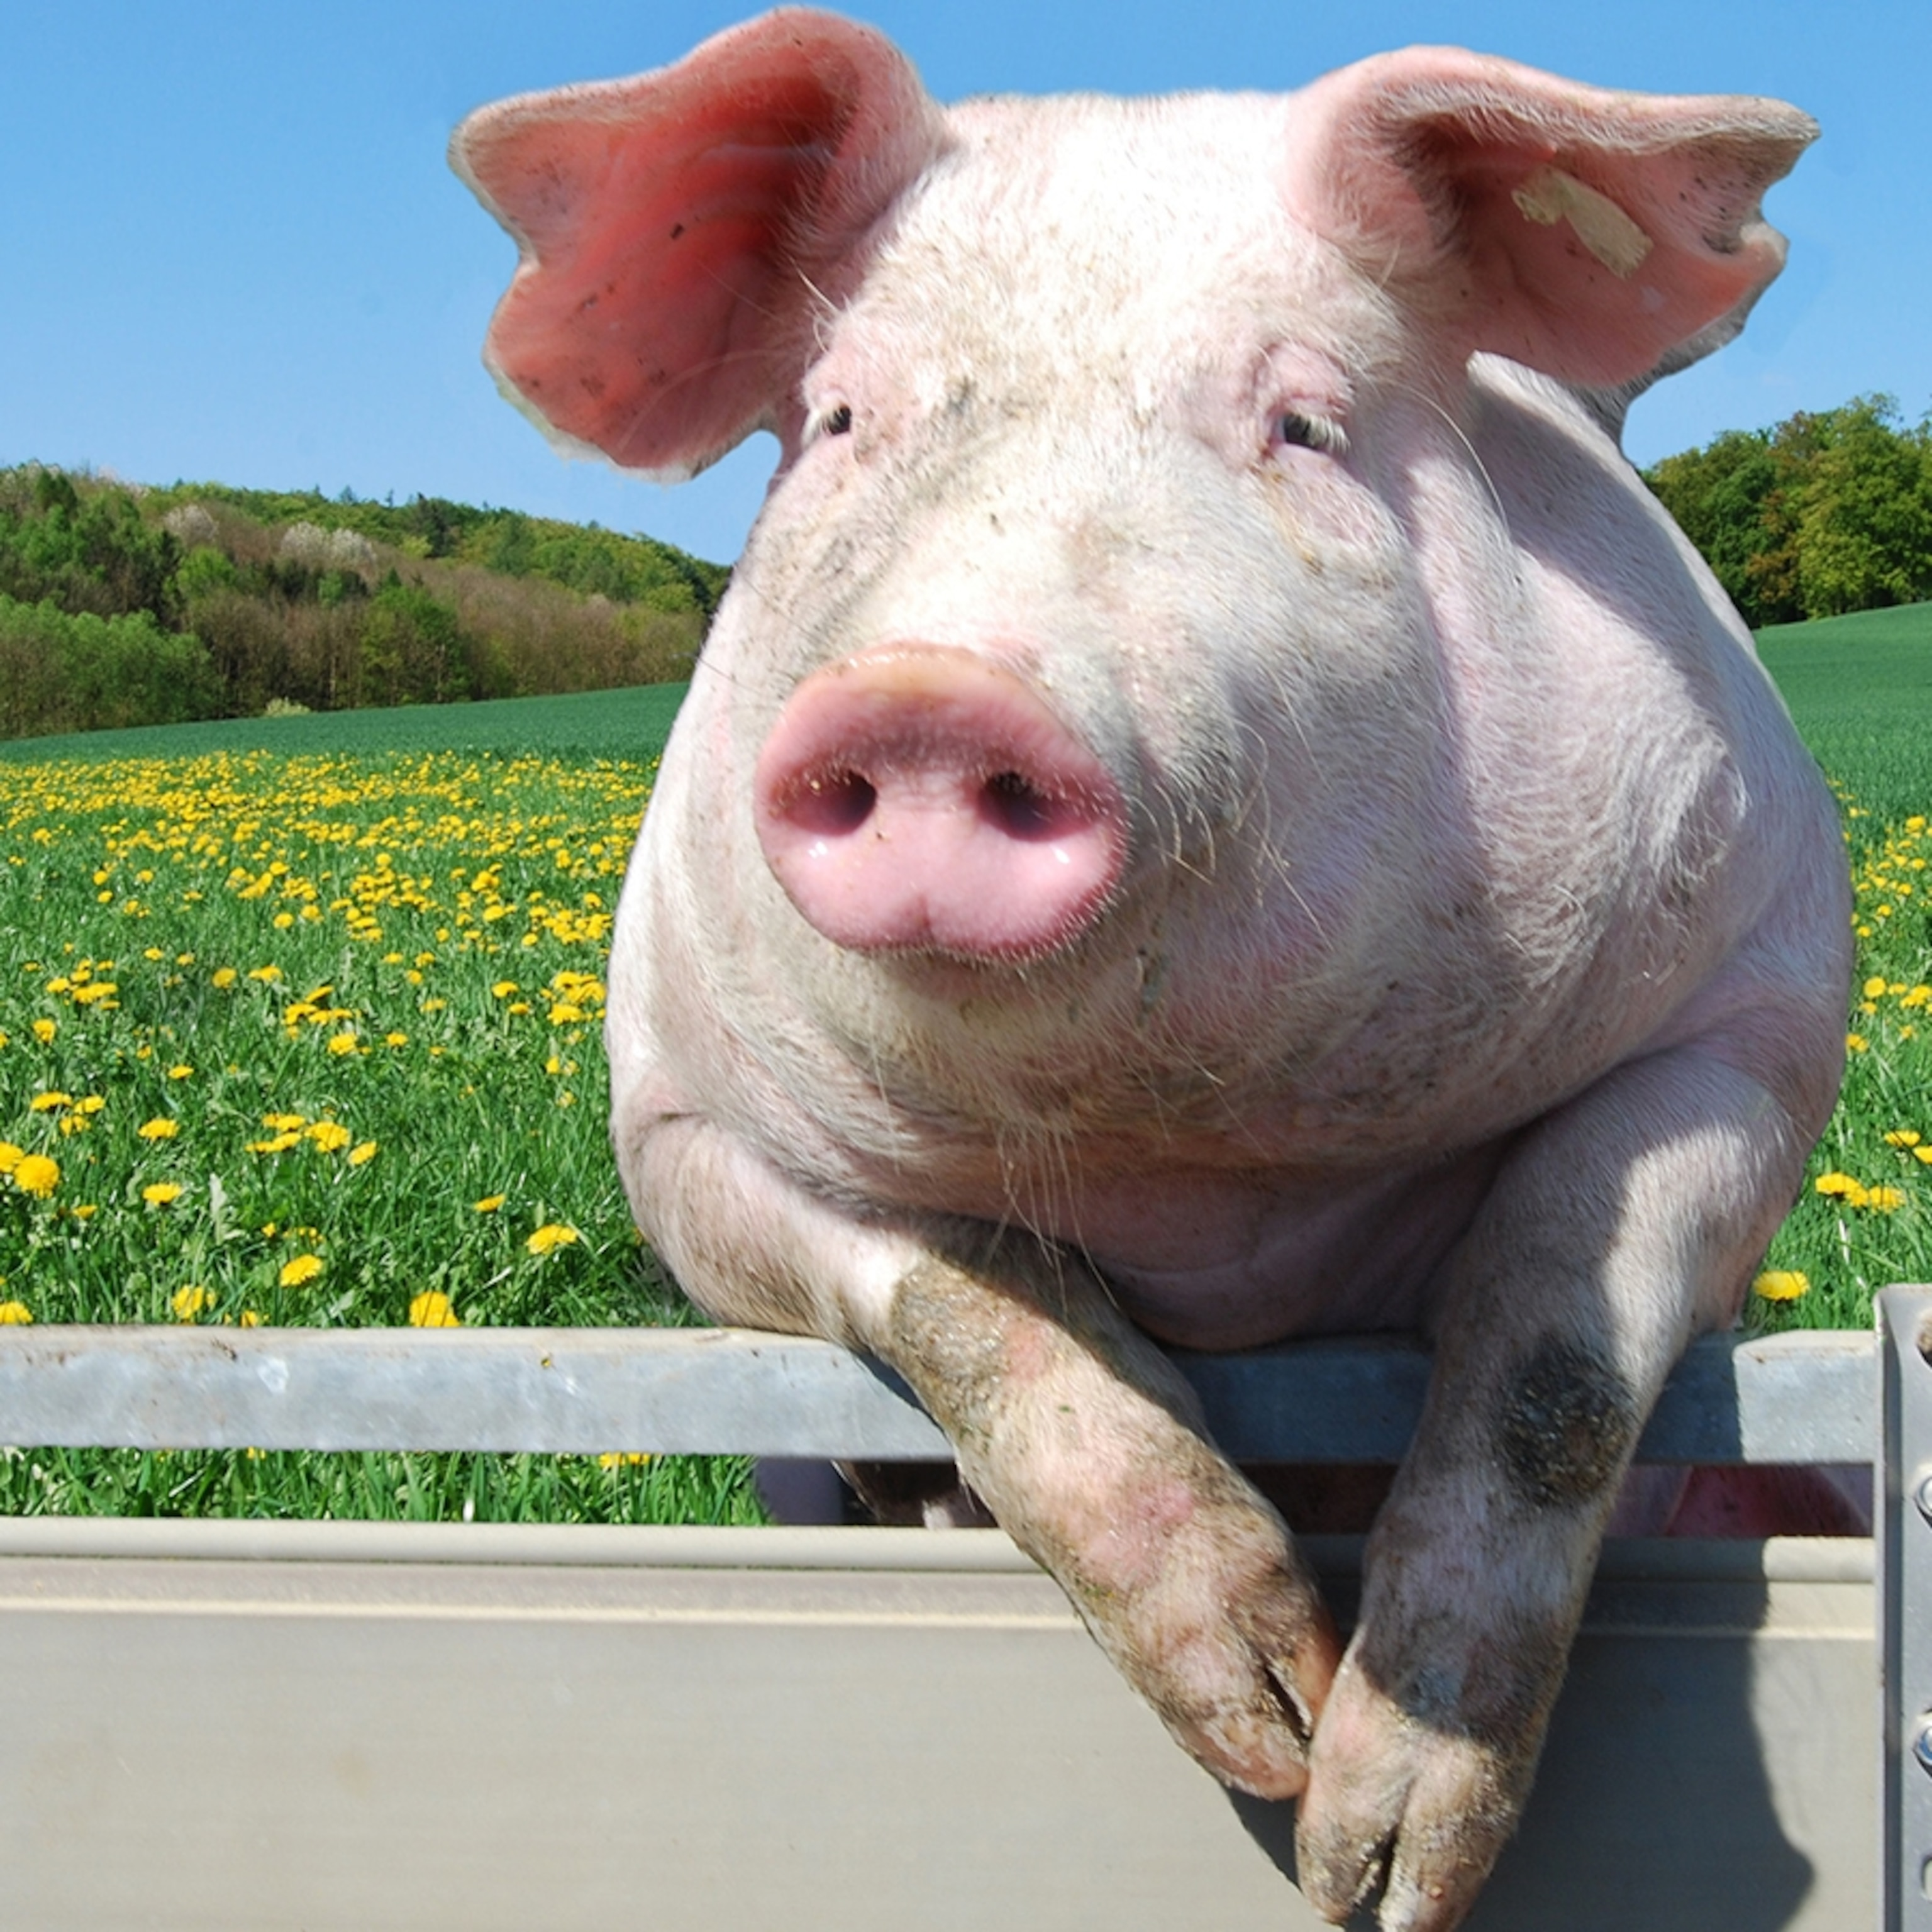
\includegraphics[width=\textwidth]{IMAGES/pep.jpg}
    \caption*{Be as happy as he is when reading this book.}
\end{figure}

\textit{%Livret réalisé par \href{https://people.epfl.ch/florentin.julien}{Florentin JULIEN}\\
It gathers all the necessary course from EPFL to be a great energy engineer.}

\newpage\phantom{blabla}
\textMark{1}

\thispagestyle{empty}
\newpage

\setcounter{tocdepth}{1}


\textMark{2}
\hypertarget{reviensSTP}{}

\tableofcontents

\newpage
%1 if course is in english, 0 otherwise
\chapter{MA1}
\includesection{convex.tex}{Convex Optimization}{1}
\includesection{electrochemistry.tex}{Electrochemistry for materials technology}{1}
\includesection{energy_conv.tex}{Energy conversion and renewable energy}{1}
\includesection{fund_elec_circuits.tex}{Fundamentals of electrical circuits and systems I}{1}
\includesection{hydro_turb.tex}{Hydraulic turbomachines}{1}
\includesection{hypowerplant.tex}{Hydropower plants : generating and pumping units}{1}
\includesection{indus_elec.tex}{Industrial electronics I}{1}
\includesection{life_cycle.tex}{Life cycle assessment in energy systems}{1}


\chapter{MA2}
\includesection{advanced_lab.tex}{Advanced lab in electrical energy system}{0}
\includesection{electromag_comp.tex}{Electromagnetic compatibility}{1}
\includesection{nrj_supply.tex}{Energy supply, economics and transition}{1}
\includesection{fundamentals_pv.tex}{Fundamentals of photovoltaic devices}{1}
\includesection{heat_pump.tex}{Heat pump systems}{1}
\includesection{hydroaccoustique.tex}{Hydroacoustic for hydropower plants}{1}
\includesection{Industrial_elec2.tex}{Industrial Electronic II}{1}
\includesection{energy_system.tex}{Energy system engineering}{1}
\includesection{ImageAnalysis.tex}{Image Analysis and Pattern Recognition}{1}
\includesection{Renewable.tex}{Renewable Energy for ME}{1}
\includesection{Water_resources.tex}{Water resources engineering and management}{1}


\includesection{no_section.tex}{No section}{0}


\chapter{MA3}
\includesection{nrj_storage.tex}{Energy storage system}{1}
\includesection{power_sys.tex}{Power system analysis}{1}

\chapter{Annex}
\includesection{matrixCalc.tex}{Matrix calculation}{1}



\end{document}